\documentclass[twoside]{book}

% Packages required by doxygen
\usepackage{fixltx2e}
\usepackage{calc}
\usepackage{doxygen}
\usepackage[export]{adjustbox} % also loads graphicx
\usepackage{graphicx}
\usepackage[utf8]{inputenc}
\usepackage{makeidx}
\usepackage{multicol}
\usepackage{multirow}
\PassOptionsToPackage{warn}{textcomp}
\usepackage{textcomp}
\usepackage[nointegrals]{wasysym}
\usepackage[table]{xcolor}

% Font selection
\usepackage[T1]{fontenc}
\usepackage[scaled=.90]{helvet}
\usepackage{courier}
\usepackage{amssymb}
\usepackage{sectsty}
\renewcommand{\familydefault}{\sfdefault}
\allsectionsfont{%
  \fontseries{bc}\selectfont%
  \color{darkgray}%
}
\renewcommand{\DoxyLabelFont}{%
  \fontseries{bc}\selectfont%
  \color{darkgray}%
}
\newcommand{\+}{\discretionary{\mbox{\scriptsize$\hookleftarrow$}}{}{}}

% Page & text layout
\usepackage{geometry}
\geometry{%
  a4paper,%
  top=2.5cm,%
  bottom=2.5cm,%
  left=2.5cm,%
  right=2.5cm%
}
\tolerance=750
\hfuzz=15pt
\hbadness=750
\setlength{\emergencystretch}{15pt}
\setlength{\parindent}{0cm}
\setlength{\parskip}{3ex plus 2ex minus 2ex}
\makeatletter
\renewcommand{\paragraph}{%
  \@startsection{paragraph}{4}{0ex}{-1.0ex}{1.0ex}{%
    \normalfont\normalsize\bfseries\SS@parafont%
  }%
}
\renewcommand{\subparagraph}{%
  \@startsection{subparagraph}{5}{0ex}{-1.0ex}{1.0ex}{%
    \normalfont\normalsize\bfseries\SS@subparafont%
  }%
}
\makeatother

% Headers & footers
\usepackage{fancyhdr}
\pagestyle{fancyplain}
\fancyhead[LE]{\fancyplain{}{\bfseries\thepage}}
\fancyhead[CE]{\fancyplain{}{}}
\fancyhead[RE]{\fancyplain{}{\bfseries\leftmark}}
\fancyhead[LO]{\fancyplain{}{\bfseries\rightmark}}
\fancyhead[CO]{\fancyplain{}{}}
\fancyhead[RO]{\fancyplain{}{\bfseries\thepage}}
\fancyfoot[LE]{\fancyplain{}{}}
\fancyfoot[CE]{\fancyplain{}{}}
\fancyfoot[RE]{\fancyplain{}{\bfseries\scriptsize Generated by Doxygen }}
\fancyfoot[LO]{\fancyplain{}{\bfseries\scriptsize Generated by Doxygen }}
\fancyfoot[CO]{\fancyplain{}{}}
\fancyfoot[RO]{\fancyplain{}{}}
\renewcommand{\footrulewidth}{0.4pt}
\renewcommand{\chaptermark}[1]{%
  \markboth{#1}{}%
}
\renewcommand{\sectionmark}[1]{%
  \markright{\thesection\ #1}%
}

% Indices & bibliography
\usepackage{natbib}
\usepackage[titles]{tocloft}
\setcounter{tocdepth}{3}
\setcounter{secnumdepth}{5}
\makeindex

% Hyperlinks (required, but should be loaded last)
\usepackage{ifpdf}
\ifpdf
  \usepackage[pdftex,pagebackref=true]{hyperref}
\else
  \usepackage[ps2pdf,pagebackref=true]{hyperref}
\fi
\hypersetup{%
  colorlinks=true,%
  linkcolor=blue,%
  citecolor=blue,%
  unicode%
}

% Custom commands
\newcommand{\clearemptydoublepage}{%
  \newpage{\pagestyle{empty}\cleardoublepage}%
}

\usepackage{caption}
\captionsetup{labelsep=space,justification=centering,font={bf},singlelinecheck=off,skip=4pt,position=top}

%===== C O N T E N T S =====

\begin{document}

% Titlepage & ToC
\hypersetup{pageanchor=false,
             bookmarksnumbered=true,
             pdfencoding=unicode
            }
\pagenumbering{alph}
\begin{titlepage}
\vspace*{7cm}
\begin{center}%
{\Large My Project }\\
\vspace*{1cm}
{\large Generated by Doxygen 1.8.13}\\
\end{center}
\end{titlepage}
\clearemptydoublepage
\pagenumbering{roman}
\tableofcontents
\clearemptydoublepage
\pagenumbering{arabic}
\hypersetup{pageanchor=true}

%--- Begin generated contents ---
\chapter{Hierarchical Index}
\section{Class Hierarchy}
This inheritance list is sorted roughly, but not completely, alphabetically\+:\begin{DoxyCompactList}
\item \contentsline{section}{open\+Gl\+Interface}{\pageref{classopenGlInterface}}{}
\begin{DoxyCompactList}
\item \contentsline{section}{bergson}{\pageref{classbergson}}{}
\end{DoxyCompactList}
\item T\+A\+B\+LE\begin{DoxyCompactList}
\item \contentsline{section}{table\+Bergson}{\pageref{classtableBergson}}{}
\end{DoxyCompactList}
\end{DoxyCompactList}

\chapter{Class Index}
\section{Class List}
Here are the classes, structs, unions and interfaces with brief descriptions\+:\begin{DoxyCompactList}
\item\contentsline{section}{\hyperlink{classbergson}{bergson} }{\pageref{classbergson}}{}
\item\contentsline{section}{\hyperlink{classopenGlInterface}{open\+Gl\+Interface} }{\pageref{classopenGlInterface}}{}
\item\contentsline{section}{\hyperlink{classtableBergson}{table\+Bergson} }{\pageref{classtableBergson}}{}
\end{DoxyCompactList}

\chapter{Class Documentation}
\hypertarget{classbergson}{}\section{bergson Class Reference}
\label{classbergson}\index{bergson@{bergson}}


Inheritance diagram for bergson\+:
\nopagebreak
\begin{figure}[H]
\begin{center}
\leavevmode
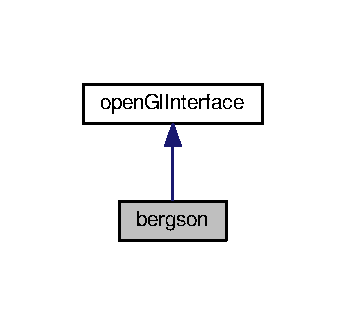
\includegraphics[width=166pt]{classbergson__inherit__graph}
\end{center}
\end{figure}


Collaboration diagram for bergson\+:
\nopagebreak
\begin{figure}[H]
\begin{center}
\leavevmode
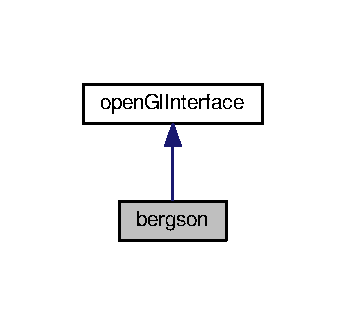
\includegraphics[width=166pt]{classbergson__coll__graph}
\end{center}
\end{figure}
\subsection*{Public Member Functions}
\begin{DoxyCompactItemize}
\item 
\mbox{\Hypertarget{classbergson_a926def93d37576874603609c418d758d}\label{classbergson_a926def93d37576874603609c418d758d}} 
{\bfseries bergson} (int argc, char $\ast$argv\mbox{[}$\,$\mbox{]})
\end{DoxyCompactItemize}
\subsection*{Static Public Member Functions}
\begin{DoxyCompactItemize}
\item 
\mbox{\Hypertarget{classbergson_a774df0ea089cb593db12e2b980b336d4}\label{classbergson_a774df0ea089cb593db12e2b980b336d4}} 
static void {\bfseries afficher\+Liste\+Dessin1} ()
\item 
\mbox{\Hypertarget{classbergson_a1d7a5125217c84b96abd7cb1793afc28}\label{classbergson_a1d7a5125217c84b96abd7cb1793afc28}} 
static void {\bfseries afficher\+Liste\+Dessin2} ()
\item 
\mbox{\Hypertarget{classbergson_a3dd5969ef6299d9902c3cce78217a430}\label{classbergson_a3dd5969ef6299d9902c3cce78217a430}} 
static void {\bfseries afficher\+Liste\+Texte} ()
\item 
\mbox{\Hypertarget{classbergson_a224c24ef264c355926da80acabcbc22f}\label{classbergson_a224c24ef264c355926da80acabcbc22f}} 
static void {\bfseries afficher\+Liste} ()
\item 
\mbox{\Hypertarget{classbergson_a4b0d0f23b70161af6f9f94e78a471aa1}\label{classbergson_a4b0d0f23b70161af6f9f94e78a471aa1}} 
static void {\bfseries interrogation} ()
\item 
\mbox{\Hypertarget{classbergson_a70cc65d6f4fbc608082935d22d98b4f9}\label{classbergson_a70cc65d6f4fbc608082935d22d98b4f9}} 
static void {\bfseries my\+\_\+handle\+\_\+key} (unsigned char key, int x, int y)
\item 
\mbox{\Hypertarget{classbergson_ac378f7da7d2406749df15840b6524d06}\label{classbergson_ac378f7da7d2406749df15840b6524d06}} 
static int {\bfseries load\+Meta\+Data} ()
\item 
\mbox{\Hypertarget{classbergson_ae436fb8b3e5602f472fd12a1e879a7f8}\label{classbergson_ae436fb8b3e5602f472fd12a1e879a7f8}} 
static int {\bfseries save\+Meta\+Data} ()
\end{DoxyCompactItemize}
\subsection*{Public Attributes}
\begin{DoxyCompactItemize}
\item 
\mbox{\Hypertarget{classbergson_af35b3141b167e275aefbd303651b2f69}\label{classbergson_af35b3141b167e275aefbd303651b2f69}} 
int {\bfseries flag\+Shot} =false
\item 
\mbox{\Hypertarget{classbergson_a5a7bcc65387a9f8f80e65ef7296ee8c7}\label{classbergson_a5a7bcc65387a9f8f80e65ef7296ee8c7}} 
int {\bfseries flag\+Blitz} =true
\end{DoxyCompactItemize}
\subsection*{Static Public Attributes}
\begin{DoxyCompactItemize}
\item 
\mbox{\Hypertarget{classbergson_aff99dc406a8877cabb93405785845697}\label{classbergson_aff99dc406a8877cabb93405785845697}} 
static string {\bfseries s\+\_\+\+Allemand}
\item 
\mbox{\Hypertarget{classbergson_a246f8e1bbc5adb5a4dd7e01a5b21ae77}\label{classbergson_a246f8e1bbc5adb5a4dd7e01a5b21ae77}} 
static string {\bfseries s\+\_\+\+Francais}
\end{DoxyCompactItemize}


The documentation for this class was generated from the following files\+:\begin{DoxyCompactItemize}
\item 
bergson.\+hpp\item 
bergson.\+cpp\item 
bergson\+Logistique.\+cpp\item 
main.\+cpp\end{DoxyCompactItemize}

\hypertarget{classopenGlInterface}{}\section{open\+Gl\+Interface Class Reference}
\label{classopenGlInterface}\index{open\+Gl\+Interface@{open\+Gl\+Interface}}


Inheritance diagram for open\+Gl\+Interface\+:
\nopagebreak
\begin{figure}[H]
\begin{center}
\leavevmode
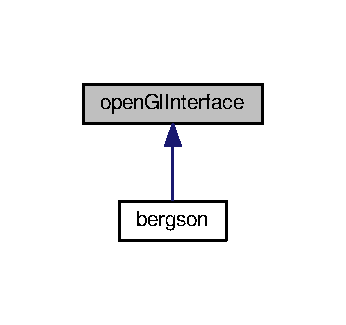
\includegraphics[width=166pt]{classopenGlInterface__inherit__graph}
\end{center}
\end{figure}
\subsection*{Public Member Functions}
\begin{DoxyCompactItemize}
\item 
\mbox{\Hypertarget{classopenGlInterface_aeba8c342b0d0f3c1810c641d2b6c50c0}\label{classopenGlInterface_aeba8c342b0d0f3c1810c641d2b6c50c0}} 
void {\bfseries init\+\_\+font} (G\+Luint base, char $\ast$f)
\item 
\mbox{\Hypertarget{classopenGlInterface_aafdfc29720767f92ad1214516ed1dae5}\label{classopenGlInterface_aafdfc29720767f92ad1214516ed1dae5}} 
void {\bfseries my\+\_\+init} (char $\ast$f)
\item 
\mbox{\Hypertarget{classopenGlInterface_ad79fa9755d5c4e6210db8a9c265791c6}\label{classopenGlInterface_ad79fa9755d5c4e6210db8a9c265791c6}} 
{\bfseries open\+Gl\+Interface} (int argc, char $\ast$argv\mbox{[}$\,$\mbox{]})
\end{DoxyCompactItemize}
\subsection*{Static Public Member Functions}
\begin{DoxyCompactItemize}
\item 
\mbox{\Hypertarget{classopenGlInterface_a8896e795148e1e7809811e8497b75913}\label{classopenGlInterface_a8896e795148e1e7809811e8497b75913}} 
static void {\bfseries attente} (void)
\item 
\mbox{\Hypertarget{classopenGlInterface_aee682263bcffbc47dd9f6df0c85c1bc0}\label{classopenGlInterface_aee682263bcffbc47dd9f6df0c85c1bc0}} 
static void {\bfseries gestion\+Liste\+\_\+rectangle} (double x1, double y1, double x2, double y2)
\item 
\mbox{\Hypertarget{classopenGlInterface_aeb8c2e01f2f2ec59d8a01fdea9450cff}\label{classopenGlInterface_aeb8c2e01f2f2ec59d8a01fdea9450cff}} 
static void {\bfseries gestion\+Liste\+\_\+rectangle\+Plein} (double x1, double y1, double x2, double y2)
\item 
\mbox{\Hypertarget{classopenGlInterface_ab53f71ec83a26e06f4b8d97b7459b6ee}\label{classopenGlInterface_ab53f71ec83a26e06f4b8d97b7459b6ee}} 
static void {\bfseries gestion\+Liste\+\_\+gestion\+Curseur} (int Sens)
\item 
\mbox{\Hypertarget{classopenGlInterface_aa686ac044c55389cc7f2b5415befbe5f}\label{classopenGlInterface_aa686ac044c55389cc7f2b5415befbe5f}} 
static void {\bfseries gestion\+Liste\+\_\+affichage\+Menu\+Horizontal} ()
\item 
\mbox{\Hypertarget{classopenGlInterface_a51a7026004c45cee6cf1d9df50e4f1e7}\label{classopenGlInterface_a51a7026004c45cee6cf1d9df50e4f1e7}} 
static void {\bfseries gestion\+Liste\+\_\+affichage\+Menu\+Vertical} ()
\item 
\mbox{\Hypertarget{classopenGlInterface_acbd69c19fc4c90a723e14797cbfbacca}\label{classopenGlInterface_acbd69c19fc4c90a723e14797cbfbacca}} 
static void {\bfseries colonne\+Concernee} (int x, int y)
\item 
\mbox{\Hypertarget{classopenGlInterface_aedf2ea6f451cce3507fbd376c82e9476}\label{classopenGlInterface_aedf2ea6f451cce3507fbd376c82e9476}} 
static int {\bfseries mot\+Concerne} (int x, int y)
\item 
\mbox{\Hypertarget{classopenGlInterface_a1ae632cac9f86be8ff949b23f8b817ff}\label{classopenGlInterface_a1ae632cac9f86be8ff949b23f8b817ff}} 
static double {\bfseries offset\+Position\+Monde\+Curseur\+Souris\+\_\+X} (double old\+Ratiox, int x, int y)
\item 
\mbox{\Hypertarget{classopenGlInterface_a86450d617b2f9bd4369a407da0a135ee}\label{classopenGlInterface_a86450d617b2f9bd4369a407da0a135ee}} 
static double {\bfseries offset\+Position\+Monde\+Curseur\+Souris\+\_\+Y} (double old\+Ratioy, int x, int y)
\item 
\mbox{\Hypertarget{classopenGlInterface_af89e7f138268d2880eb18ba964f5a7f8}\label{classopenGlInterface_af89e7f138268d2880eb18ba964f5a7f8}} 
static void {\bfseries print\+\_\+string} (G\+Luint base, const char $\ast$s)
\item 
\mbox{\Hypertarget{classopenGlInterface_a791f03e629a6ba0bace620d44709fe2b}\label{classopenGlInterface_a791f03e629a6ba0bace620d44709fe2b}} 
static void {\bfseries my\+\_\+reshape} (int w, int h)
\item 
\mbox{\Hypertarget{classopenGlInterface_a8119b9e6ff26179450ad9d4844d08a26}\label{classopenGlInterface_a8119b9e6ff26179450ad9d4844d08a26}} 
static void {\bfseries my\+\_\+motion\+Mouse} (int x, int y)
\item 
\mbox{\Hypertarget{classopenGlInterface_a487b51f6970788f69ca9465ba21be54f}\label{classopenGlInterface_a487b51f6970788f69ca9465ba21be54f}} 
static void {\bfseries my\+\_\+mouse} (int button, int state, int x, int y)
\item 
\mbox{\Hypertarget{classopenGlInterface_a0d1a23a768cc818139631637ed2e01cf}\label{classopenGlInterface_a0d1a23a768cc818139631637ed2e01cf}} 
static int {\bfseries load\+Meta\+Data} ()
\item 
\mbox{\Hypertarget{classopenGlInterface_a4dd9bf76640c23212e9c3d05d23e9a3b}\label{classopenGlInterface_a4dd9bf76640c23212e9c3d05d23e9a3b}} 
static int {\bfseries save\+Meta\+Data} ()
\end{DoxyCompactItemize}
\subsection*{Public Attributes}
\begin{DoxyCompactItemize}
\item 
\mbox{\Hypertarget{classopenGlInterface_af2e6e6db6a8a3a37b755ad499abbc2aa}\label{classopenGlInterface_af2e6e6db6a8a3a37b755ad499abbc2aa}} 
char {\bfseries window\+\_\+title} \mbox{[}256\mbox{]}
\item 
\mbox{\Hypertarget{classopenGlInterface_a839ac2fcf0e349195b01128e0668e7b7}\label{classopenGlInterface_a839ac2fcf0e349195b01128e0668e7b7}} 
char {\bfseries font\+\_\+name} \mbox{[}256\mbox{]}
\end{DoxyCompactItemize}
\subsection*{Static Public Attributes}
\begin{DoxyCompactItemize}
\item 
\mbox{\Hypertarget{classopenGlInterface_a3d916ba240cfc3bde773f3db8d0ed536}\label{classopenGlInterface_a3d916ba240cfc3bde773f3db8d0ed536}} 
static string {\bfseries file\+Name}
\item 
\mbox{\Hypertarget{classopenGlInterface_a96dc191c263729869fd0a2b90fcbcccc}\label{classopenGlInterface_a96dc191c263729869fd0a2b90fcbcccc}} 
static string {\bfseries file\+Name2}
\item 
\mbox{\Hypertarget{classopenGlInterface_a30b03223a4dd046bf817de6b29cc7015}\label{classopenGlInterface_a30b03223a4dd046bf817de6b29cc7015}} 
static string {\bfseries file\+Name\+Liste}
\item 
\mbox{\Hypertarget{classopenGlInterface_a643c200dd079c5e10142df320491daac}\label{classopenGlInterface_a643c200dd079c5e10142df320491daac}} 
static float {\bfseries pos} \mbox{[}2\mbox{]} = \{0.\+0 , 0.\+0\}
\item 
\mbox{\Hypertarget{classopenGlInterface_a9ce89ad19c8eef5a83916c9b02601e84}\label{classopenGlInterface_a9ce89ad19c8eef5a83916c9b02601e84}} 
static float {\bfseries ratio} \mbox{[}2\mbox{]} = \{1.\+0, 1.\+0\}
\item 
\mbox{\Hypertarget{classopenGlInterface_a5979006cb0d277e2a1171a69d36e7b0f}\label{classopenGlInterface_a5979006cb0d277e2a1171a69d36e7b0f}} 
static float {\bfseries old} \mbox{[}2\mbox{]} =\{0.\+0, 0.\+0\}
\item 
\mbox{\Hypertarget{classopenGlInterface_a9754eb99954cf48d6bbfb150ba273d2e}\label{classopenGlInterface_a9754eb99954cf48d6bbfb150ba273d2e}} 
static float {\bfseries offsety} =0.\+0
\item 
\mbox{\Hypertarget{classopenGlInterface_a22f96ee0a9a0e10fc7149ab24629e2d7}\label{classopenGlInterface_a22f96ee0a9a0e10fc7149ab24629e2d7}} 
static int {\bfseries pause} =false
\item 
\mbox{\Hypertarget{classopenGlInterface_a9e9acd84308f7f410d29380057e09713}\label{classopenGlInterface_a9e9acd84308f7f410d29380057e09713}} 
static int {\bfseries left\+State} =0
\item 
\mbox{\Hypertarget{classopenGlInterface_acdd9530d760aff3714cc4212e5b781b7}\label{classopenGlInterface_acdd9530d760aff3714cc4212e5b781b7}} 
static int {\bfseries right\+State} =0
\item 
\mbox{\Hypertarget{classopenGlInterface_aa1da903bf927fa54e185f8ff3c495dd4}\label{classopenGlInterface_aa1da903bf927fa54e185f8ff3c495dd4}} 
static int {\bfseries nearest\+Table\+Index} =-\/1
\item 
\mbox{\Hypertarget{classopenGlInterface_a6f7d4585d7c035ad2b47f922f52b26ec}\label{classopenGlInterface_a6f7d4585d7c035ad2b47f922f52b26ec}} 
static int {\bfseries posx\+Curseur}
\item 
\mbox{\Hypertarget{classopenGlInterface_ac0eaa737f4b46c8b599efde951de7af5}\label{classopenGlInterface_ac0eaa737f4b46c8b599efde951de7af5}} 
static G\+Luint {\bfseries font\+\_\+base} = 0
\item 
\mbox{\Hypertarget{classopenGlInterface_a97941ddeb831dc62993606e953124eba}\label{classopenGlInterface_a97941ddeb831dc62993606e953124eba}} 
static vector$<$ \hyperlink{classtableBergson}{table\+Bergson} $>$ {\bfseries Bdd}
\item 
\mbox{\Hypertarget{classopenGlInterface_aa3e67775fec268a61844158466bb4b61}\label{classopenGlInterface_aa3e67775fec268a61844158466bb4b61}} 
static T\+A\+B\+LE {\bfseries ma\+Liste\+De\+Liste}
\end{DoxyCompactItemize}


The documentation for this class was generated from the following files\+:\begin{DoxyCompactItemize}
\item 
open\+Gl.\+hpp\item 
main.\+cpp\item 
open\+Gl.\+cpp\item 
open\+Gl\+Windows.\+cpp\end{DoxyCompactItemize}

\hypertarget{classtableBergson}{}\section{table\+Bergson Class Reference}
\label{classtableBergson}\index{table\+Bergson@{table\+Bergson}}


Inheritance diagram for table\+Bergson\+:
\nopagebreak
\begin{figure}[H]
\begin{center}
\leavevmode
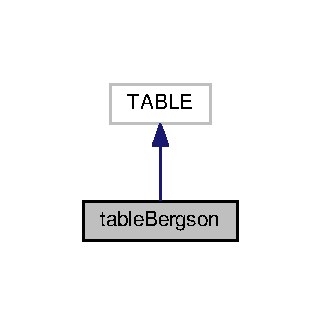
\includegraphics[width=154pt]{classtableBergson__inherit__graph}
\end{center}
\end{figure}


Collaboration diagram for table\+Bergson\+:
\nopagebreak
\begin{figure}[H]
\begin{center}
\leavevmode
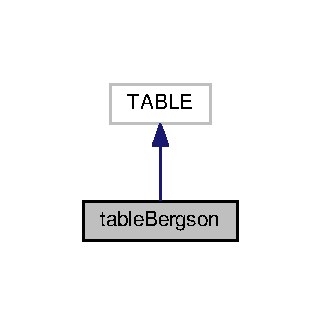
\includegraphics[width=154pt]{classtableBergson__coll__graph}
\end{center}
\end{figure}
\subsection*{Public Attributes}
\begin{DoxyCompactItemize}
\item 
\mbox{\Hypertarget{classtableBergson_adaec1cc9fa66934fb753b73cf1cea6c8}\label{classtableBergson_adaec1cc9fa66934fb753b73cf1cea6c8}} 
int {\bfseries flag\+Visible}
\item 
\mbox{\Hypertarget{classtableBergson_a3de79075c33d5fdfada9f9d1ea7b42f7}\label{classtableBergson_a3de79075c33d5fdfada9f9d1ea7b42f7}} 
int {\bfseries flag\+Question\+Visible}
\item 
\mbox{\Hypertarget{classtableBergson_afd6b8a993aceba9061b8acd499ee0c19}\label{classtableBergson_afd6b8a993aceba9061b8acd499ee0c19}} 
int {\bfseries flag\+Memo\+Visible}
\item 
\mbox{\Hypertarget{classtableBergson_ab0415c47c341dcaf315cc3d9c910304f}\label{classtableBergson_ab0415c47c341dcaf315cc3d9c910304f}} 
double {\bfseries pos} \mbox{[}2\mbox{]}
\item 
\mbox{\Hypertarget{classtableBergson_a855fb30d561c14e0043b82eb34378a39}\label{classtableBergson_a855fb30d561c14e0043b82eb34378a39}} 
float {\bfseries color} \mbox{[}4\mbox{]}
\item 
\mbox{\Hypertarget{classtableBergson_afcddc43fc5e2e77043f00cec9b61833c}\label{classtableBergson_afcddc43fc5e2e77043f00cec9b61833c}} 
string {\bfseries filename}
\end{DoxyCompactItemize}


The documentation for this class was generated from the following file\+:\begin{DoxyCompactItemize}
\item 
open\+Gl.\+hpp\end{DoxyCompactItemize}

%--- End generated contents ---

% Index
\backmatter
\newpage
\phantomsection
\clearemptydoublepage
\addcontentsline{toc}{chapter}{Index}
\printindex

\end{document}
